\subsection{Hyperboloids}
\noindent
A hyperboloid looks like a hyperbola that has been rotated and extruded about its center. It is also radially symmetric with circular level curves. Paraboloids have the form 
\begin{equation*}
	d = \pm \frac{x^2}{a^2} \pm \frac{y^2}{b^2} \pm \frac{z^2}{c^2}	
\end{equation*}
where one sign is different from the others. Depending on the signs and the value of $d$, one can get a hyperboloid of one sheet, two sheets, or a cone.
\subsubsection{Hyperboloids of One Sheet}
\noindent
A hyperboloid of one sheet has 2 +'s and 1 - in its equation. It is one fully connected surface.

\begin{figure}[H]
	\centering
	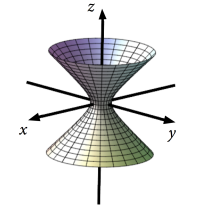
\includegraphics[width=0.33\textwidth]{./Images/differentialMultivariableCalculus/one_sheet.png}
	\caption{A hyperboloid of one sheet}
\end{figure}
\subsubsection{Hyperboloids of Two Sheets}
\noindent
A hyperboloid of two sheets has 2 -'s and 1 + in its equation. It is made up of two disconnected, mirror image, surfaces.

[INSERT IMAGE]
\subsubsection{Cone}
A cone is a transition state between one-sheet and two-sheet hyperboloids.
When the constant term in the hyperboloid's equation is 0, the top and bottom surfaces are only connected at a single point.

\begin{figure}[H]
	\centering
	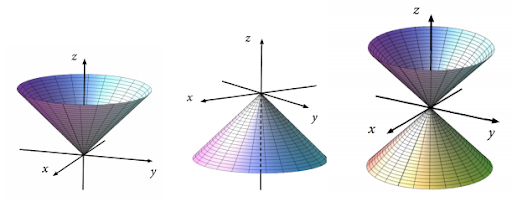
\includegraphics[width=0.8\textwidth]{./Images/differentialMultivariableCalculus/cones.png}
	\caption{Cones}
\end{figure}